%% ============================================================================
%% Manuscrito LLMTDD — TDDMachine (BORRADOR EN ESPAÑOL para revisión interna)
%% Plantilla no oficial Enfoque UTE (formato IEEE, 2026).
%% NOTA: Enfoque UTE exige el envío final en INGLÉS con resumen en español.
%%       Este .tex es el borrador en español; la versión en inglés se derivará
%%       de este una vez aprobado el contenido.
%%
%% Compilación (Windows, MiKTeX/TeX Live):
%%   pdflatex main.tex
%%   bibtex   main
%%   pdflatex main.tex
%%   pdflatex main.tex
%% ============================================================================

\documentclass[10pt,journal,twoside,letterpaper]{IEEEtran}

%% ------------------ Codificación e idiomas ------------------
\usepackage[T1]{fontenc}
\usepackage[utf8]{inputenc}
%% Idioma principal "english" (va en ÚLTIMO lugar): garantiza etiquetas
%% estructurales IEEE en inglés y marcadores PDF (hyperref) estables con
%% caracteres acentuados. El cuerpo se compone en español y activa las reglas
%% de partición de palabras del español mediante \selectlanguage al inicio del
%% cuerpo; el resumen y las palabras clave en español se proveen con los
%% entornos personalizados \resumen y \palabrasclave.
\usepackage[spanish,english]{babel}
\shorthandoff{.<>}

%% ------------------ Geometría (US Letter, estilo IEEE de dos columnas) -------
%% Márgenes equilibrados y separación de columnas estrecha (0.25in) al estilo
%% IEEE Transactions, para columnas más anchas y una justificación más limpia.
\usepackage[
letterpaper,
top=0.75in,
bottom=0.95in,
left=0.62in,
right=0.62in,
columnsep=0.25in,
headsep=12pt,
headheight=14pt,
footskip=28pt
]{geometry}

%% ------------------ Paquetes de contenido ------------------
\usepackage{graphicx}
\usepackage{amsmath,amssymb,amsfonts}
\usepackage{array}
\usepackage{booktabs}
\usepackage{multirow}
\usepackage{textcomp}
\usepackage{xcolor}
\usepackage{url}
\usepackage[hidelinks]{hyperref}
\usepackage{cite}
\usepackage{orcidlink}
\usepackage[protrusion=true,expansion=true]{microtype} % justificación más limpia

%% Etiquetas estructurales en inglés (estilo IEEE de Enfoque UTE), aunque el
%% idioma principal del cuerpo sea el español. Se aplica al iniciar el documento
%% para prevalecer sobre las definiciones de babel-spanish.
\AtBeginDocument{%
	\renewcommand{\abstractname}{Abstract}%
	\renewcommand{\figurename}{Fig.}%
	\renewcommand{\tablename}{TABLE}%
	\renewcommand{\refname}{References}%
	\renewcommand{\bibname}{References}%
}

%% ------------------ Ajustes de figuras y tablas ------------------
\graphicspath{{./figures/}{./}}
\renewcommand{\arraystretch}{1.2}

%% ------------------ Logo institucional (primera página) ------------------
\usepackage{fancyhdr}
%% El logo se coloca en la cabecera de la portada como una caja de ALTURA CERO
%% (\smash), de modo que NO reserve espacio y no empuje el cuerpo hacia abajo;
%% así el margen inferior de la portada coincide con el del resto del documento.
\fancypagestyle{enfoqueutefirstpage}{%
	\fancyhf{}
	\renewcommand{\headrulewidth}{0pt}
	\renewcommand{\footrulewidth}{0pt}
	\fancyhead[C]{%
		\smash{\raisebox{-0.35in}{
\includegraphics[width=1.9in]{enfoque_ute_logo.png}}}%
	}
	\setlength{\headheight}{14pt}
}

%% ------------------ Bloques de resumen y palabras clave en español ------------------
\newenvironment{resumen}{%
	\vspace{0.3em}
	\noindent\normalfont\small\itshape\textbf{Resumen}\hspace{0.5em}\textmd{---}\hspace{0.3em}%
	\ignorespaces
}{%
	\par\vspace{0.3em}%
}
\newcommand{\palabrasclave}[1]{%
	\vspace{0.2em}
	\noindent\small\textit{Palabras Clave}~---~#1
	\par\vspace{0.4em}
}
\newcommand{\seccionfunding}[1]{%
	\vspace{0.6em}
	\noindent\textsc{Funding}
	\par\vspace{0.2em}
	\small #1
	\par
}
\newcommand{\seccionconflicto}[1]{%
	\vspace{0.6em}
	\noindent\textsc{Conflict of Interest}
	\par\vspace{0.2em}
	\small #1
	\par
}
\newcommand{\seccioniadeclaracion}[1]{%
	\vspace{0.6em}
	\noindent\textsc{Artificial Intelligence Statement}
	\par\vspace{0.2em}
	\small #1
	\par
}
\newcommand{\seccionetica}[1]{%
	\vspace{0.6em}
	\noindent\textsc{Ethics and Informed Consent}
	\par\vspace{0.2em}
	\small #1
	\par
}

%% ============================================================================
%% METADATOS DEL ARTÍCULO
%% ============================================================================
\author{%
	Gleiston~Guerrero-Ulloa\textsuperscript{1,2}~\orcidlink{0000-0001-5990-2357},
	Kerly~M.~Triana-Arrieta\textsuperscript{1},
	Efraín~Díaz-Macías\textsuperscript{1}~\orcidlink{0000-0003-4087-029X},
	Carlos~Rodríguez-Domínguez\textsuperscript{2,3}~\orcidlink{0000-0001-5626-3115},
	and~Miguel~J.~Hornos\textsuperscript{2}~\orcidlink{0000-0001-5722-9816}%
	\thanks{\textsuperscript{1}Facultad de Ciencias de la Computación, Universidad Técnica Estatal de Quevedo (UTEQ), Quevedo 120501, Los Ríos, Ecuador. \textsuperscript{2}Departamento de Ingeniería del Software, Universidad de Granada, 18071 Granada, España. \textsuperscript{3}Centro de Investigación de Tecnologías de la Información y Comunicación (CITIC), Universidad de Granada, 18071 Granada, España.}%
	\thanks{\emph{Autor de correspondencia:} C. Rodríguez-Domínguez (correo: carlosrodriguez@ugr.es).}%
}

\markboth{Enfoque UTE (manuscrito en revisión), 2026}%
{Guerrero-Ulloa \MakeLowercase{\textit{et~al.}}: Generación del estado inicial de pruebas TDD mediante LLM}

%% ============================================================================
%% CUERPO DEL ARTÍCULO
%% ============================================================================
\begin{document}
	
	\IEEEoverridecommandlockouts
	\pretolerance=10000
	
	\title{TDDMachine: generación automática del estado inicial de pruebas para Desarrollo Guiado por Pruebas mediante un modelo de lenguaje de gran escala}
	
	\maketitle
	\thispagestyle{enfoqueutefirstpage}
	
	\begin{abstract}
		The manual creation of test cases remains a laborious, repetitive and error-prone activity, and empirical evidence shows that developers test far less than they believe, treating testing as a low-value chore; yet Test-Driven Development (TDD), in which tests are written before production code, is associated with 40--90\% lower defect density at the cost of only a modest increase in initial development effort. This paper presents TDDMachine, a Computer-Aided Software Engineering (CASE) tool that automates the generation of the initial test state (the \emph{Red} stage of the TDD cycle) from structured specifications---functional requirements, use cases and user stories---using the Claude 3.5 Sonnet large language model. The requirements were derived from a systematic literature review of 108 primary studies; the technology stack (React~18, Django~4.2, PostgreSQL~15, Docker) was chosen through weighted multi-criteria evaluation; and generated \texttt{pytest} scripts are syntactically validated through Python Abstract Syntax Tree analysis. The tool was evaluated with 25~participants using the System Usability Scale (SUS) and the Technology Acceptance Model (TAM), and with 10~experts who assessed test quality through a structured rubric. TDDMachine produced valid scripts in 91.4\% of attempts, reached a mean expert-rated quality of 4.08/5.0, obtained a SUS score of 74.82/100 (``Good''), and exceeded the technology-acceptance threshold in all four TAM constructs. The results provide empirical evidence that structured, LLM-assisted generation of the TDD initial state is both feasible and well accepted.
	\end{abstract}
	
	\begin{IEEEkeywords}
		CASE tool; automated test generation; generative artificial intelligence; large language models; Test-Driven Development; pytest; software quality assurance; requirements engineering.
	\end{IEEEkeywords}
	
	\begin{resumen}
		La creación manual de casos de prueba sigue siendo una tarea laboriosa, repetitiva y propensa a errores, y la evidencia empírica muestra que los desarrolladores prueban mucho menos de lo que creen, percibiendo la escritura de pruebas como una carga de bajo valor; sin embargo, el Desarrollo Guiado por Pruebas (TDD), en el que las pruebas se escriben antes que el código de producción, se asocia con una reducción de la densidad de defectos del 40--90\,\% a cambio de un incremento moderado del esfuerzo inicial. Este artículo presenta TDDMachine, una herramienta CASE que automatiza la generación del estado inicial de las pruebas (la etapa \emph{Red} del ciclo TDD) a partir de especificaciones estructuradas ---requisitos funcionales, casos de uso e historias de usuario--- mediante el modelo de lenguaje de gran escala Claude 3.5 Sonnet. Los requisitos se derivaron de una revisión sistemática de 108 estudios primarios; la pila tecnológica (React~18, Django~4.2, PostgreSQL~15, Docker) se seleccionó mediante evaluación multicriterio ponderada; y los scripts \texttt{pytest} generados se validan sintácticamente mediante análisis del árbol sintáctico abstracto de Python. La herramienta se evaluó con 25 participantes mediante los instrumentos SUS y TAM, y con 10 expertos que valoraron la calidad de las pruebas mediante una rúbrica estructurada. TDDMachine produjo scripts válidos en el 91,4\,\% de los intentos, alcanzó una calidad media evaluada por expertos de 4,08/5,0, obtuvo un puntaje SUS de 74,82/100 (``Bueno'') y superó el umbral de aceptación tecnológica en los cuatro constructos TAM. Los resultados aportan evidencia empírica de que la generación estructurada del estado inicial TDD asistida por LLM es viable y bien aceptada.
	\end{resumen}
	
	\palabrasclave{herramienta CASE; generación automática de pruebas; inteligencia artificial generativa; modelos de lenguaje de gran escala; Desarrollo Guiado por Pruebas; pytest; aseguramiento de calidad; ingeniería de requisitos.}
	
	%% A partir de aquí el CUERPO usa la partición de palabras del español.
	%% Se reafirman las etiquetas IEEE en inglés tras el cambio de idioma.
	\selectlanguage{spanish}
	\shorthandoff{.<>"}
	\renewcommand{\figurename}{Fig.}
	\renewcommand{\tablename}{TABLE}
	\renewcommand{\refname}{References}
	\renewcommand{\bibname}{References}
	
	%% ------------------------------------------------------------------------
	\section{Introducción}
	\label{sec:introduccion}
	
	\IEEEPARstart{L}{as} pruebas de software constituyen una actividad transversal del ciclo de vida del desarrollo, responsable de verificar la funcionalidad, la estabilidad y la confiabilidad del código antes de su puesta en producción; sin embargo, su elaboración manual continúa siendo una tarea laboriosa, repetitiva y susceptible a errores, especialmente en entornos ágiles donde los ciclos de entrega son cortos y los requisitos cambian con frecuencia \cite{lukasczyk2023empirical,wang2024survey}.
	
	Esta carga explica una tensión bien documentada en la práctica profesional: aunque las pruebas son reconocidas como esenciales, los desarrolladores tienden a percibirlas como una actividad tediosa y de bajo valor inmediato, que compite con la escritura de funcionalidad. La evidencia empírica es contundente al respecto: el estudio de campo de Beller et~al., basado en la instrumentación del entorno de desarrollo de miles de programadores, demostró que estos dedican a las pruebas mucho menos tiempo del que ellos mismos estiman, y que una fracción considerable de sesiones de desarrollo transcurre sin ejecutar una sola prueba \cite{beller2015test}. En la misma línea, la encuesta de Straubinger y Fraser reporta que una proporción significativa de desarrolladores considera la escritura de pruebas como una labor poco atractiva y la posterga sistemáticamente frente a otras tareas \cite{straubinger2023survey}. En conjunto, estos trabajos sustentan la percepción, extendida en la industria, de que escribir pruebas es una inversión de tiempo cuyo retorno no siempre resulta evidente para quien las redacta.
	
	La evidencia sobre resultados de proyecto, no obstante, apunta en sentido contrario cuando las pruebas se anticipan al código. El Desarrollo Guiado por Pruebas (\emph{Test-Driven Development}, TDD) invierte el orden tradicional de codificación: primero se escribe una prueba que falla porque el código aún no existe (etapa \emph{Red}), luego se implementa el código mínimo para que la prueba pase (etapa \emph{Green}) y, por último, se refactoriza conservando las pruebas en verde (etapa \emph{Refactor}) \cite{beck2003tdd}. El estudio industrial de Nagappan et~al. en cuatro equipos de Microsoft e IBM documentó que la densidad de defectos previa a la liberación disminuyó entre un 40\,\% y un 90\,\% respecto de proyectos comparables que no aplicaron TDD, a cambio de un incremento del tiempo inicial de desarrollo de apenas 15\,\% a 35\,\% \cite{nagappan2008tdd}. El metaanálisis de Rafique y Mišić confirma una mejora significativa de la calidad externa asociada al TDD, y el experimento controlado de Erdogmus et~al. sobre el enfoque \emph{test-first} evidenció ganancias de productividad atribuibles a la anticipación de las pruebas \cite{rafique2013meta,erdogmus2005testfirst}. La lectura conjunta de estos resultados es que un software construido a partir de sus pruebas tiene mayor probabilidad de cumplir las funcionalidades comprometidas dentro de los plazos previstos, y que la fase inicial de explotación ---aquella en la que el equipo debe corregir defectos detectados tras la entrega--- resulta notablemente más reducida que en un software cuyas pruebas se escribieron después de construir el código.
	
	El momento del ciclo de vida en que se escriben las pruebas es, por tanto, determinante. En el enfoque tradicional \emph{test-last}, las pruebas se redactan una vez implementada la funcionalidad, con lo que actúan como verificación a posteriori y heredan las decisiones de diseño ya tomadas; en el enfoque \emph{test-first} que promueve el TDD, en cambio, las pruebas se escriben antes del código de producción y operan como especificación ejecutable que guía el diseño \cite{beck2003tdd,erdogmus2005testfirst}. La ingeniería de requisitos ofrece el punto de partida idóneo para esta anticipación: cuando los requisitos funcionales, casos de uso e historias de usuario se documentan de forma estructurada conforme a estándares como ISO/IEC/IEEE~29148, sus criterios de aceptación son directamente transformables en condiciones de prueba verificables \cite{iso29148}. El reto práctico es que redactar esas pruebas iniciales desde requisitos, y hacerlo antes de escribir código, exige un esfuerzo cognitivo y una experiencia en \emph{testing} de los que muchos equipos carecen, lo que limita la adopción del TDD pese a sus beneficios demostrados \cite{ghafari2020inconclusive}.
	
	Ante retos de esta naturaleza, la ingeniería de software ha comenzado a incorporar inteligencia artificial generativa para automatizar tareas tradicionalmente manuales. Las revisiones sistemáticas más recientes documentan que los modelos de lenguaje de gran escala (\emph{Large Language Models}, LLM) se aplican con métricas de éxito medibles a lo largo de numerosos procesos del ciclo de vida ---generación y compleción de código, resumen y traducción de programas, reparación de defectos y elicitación de requisitos, entre otros--- y no solo a la fase de pruebas \cite{hou2024llm4se,carleton2024genai}. Esta tendencia se refleja también en la producción regional: en \emph{Enfoque UTE} se han publicado revisiones y estudios que reportan la aplicación de técnicas de aprendizaje automático y profundo a problemas de ingeniería con indicadores cuantitativos de desempeño, desde la clasificación mediante redes neuronales artificiales \cite{molina2024ann} hasta el ajuste automático de ancho de banda en redes inalámbricas \cite{carrillo2025ai} o la integración de IoT e IA en la agricultura \cite{basurto2026iotai}. En el ámbito específico del \emph{testing}, los LLM han mostrado capacidad para interpretar especificaciones en lenguaje natural y sintetizar casos de prueba estructurados y ejecutables, con tasas de éxito reportadas que varían según la calidad de la especificación de entrada \cite{wang2024survey,yang2024evaluation,rehan2025harnessing,bhatia2024unit,korraprolu2025testcase,takerngsaksiri2025pytester}.
	
	Las herramientas basadas en IA para generación de pruebas presentan, sin embargo, ventajas y limitaciones que conviene contrastar con la propuesta de este trabajo. \emph{ChatUniTest} \cite{chen2024chatunitest}, \emph{TestSpark} \cite{sapozhnikov2024testspark} y \emph{Pynguin} \cite{lukasczyk2022pynguin} generan pruebas unitarias con notable eficacia, pero lo hacen a partir del código fuente preexistente, por lo que operan de forma natural en un esquema \emph{test-last} e integradas a entornos de desarrollo; \emph{Pytester} \cite{takerngsaksiri2025pytester} sí traduce descripciones textuales a casos de prueba, aunque sin gestión estructurada de requisitos ni control del estado del ciclo. La ventaja de estas herramientas es su madurez y su cobertura, y su principal limitación, de cara al TDD, es que presuponen la existencia del código que la metodología precisamente propone escribir después de la prueba. La propuesta de este trabajo, denominada TDDMachine, se sitúa deliberadamente aguas arriba: es una herramienta CASE (\emph{Computer-Aided Software Engineering}) que interviene de manera exclusiva en la transición \emph{Red}$\rightarrow$\emph{Green} del ciclo TDD, generando el script de prueba en Python con \texttt{pytest} a partir de especificaciones estructuradas, para entregar al equipo de desarrollo el punto de partida sobre el cual escribir el código de producción mínimo. La solución se desarrolló derivando sus requisitos de una revisión sistemática de la literatura, seleccionando su pila tecnológica (React~18, Django~4.2, PostgreSQL~15 y despliegue en contenedores Docker) mediante evaluación multicriterio ponderada, e integrando el modelo Claude 3.5 Sonnet a través de un constructor de \emph{prompts} estructurados y un validador que verifica la sintaxis del código generado mediante el árbol sintáctico abstracto (AST) de Python. Para su comprobación se diseñaron dos estudios acordes con ese alcance: un estudio de usabilidad y aceptación tecnológica con 25 participantes, mediante los instrumentos SUS y TAM, y un estudio de calidad de las pruebas generadas con 10 expertos, mediante una rúbrica estructurada.
	
	Las contribuciones de este trabajo son tres. Primera, TDDMachine, una herramienta CASE que integra en un único flujo la captura estructurada de tres tipos de especificación ---requisitos funcionales, casos de uso e historias de usuario---, la generación del estado inicial de las pruebas mediante un LLM y la validación sintáctica del código generado mediante el AST de Python, brecha que ninguna de las herramientas del estado del arte cubre de forma integrada. Segunda, una revisión sistemática de 108 estudios primarios que caracteriza los estándares y notaciones para estructurar los requisitos y su relación con la generación automática de pruebas, y que fundamenta el diseño de la herramienta. Tercera, evidencia empírica de la viabilidad y la aceptación de la propuesta, obtenida mediante un estudio de usabilidad y aceptación tecnológica con 25 participantes y un estudio de calidad de las pruebas con 10 expertos.
	
	El resto del artículo se organiza como sigue. La Sección~\ref{sec:trabajos} presenta una breve revisión sistemática de la literatura, conducida según los lineamientos de Kitchenham, que sitúa la contribución frente al estado del arte. La Sección~\ref{sec:metodologia} describe la metodología de desarrollo y evaluación. La Sección~\ref{sec:resultados} reporta los resultados de generación, usabilidad, aceptación y calidad. La Sección~\ref{sec:discusion} discute los hallazgos frente a los objetivos y trabajos previos y expone las amenazas a la validez. Finalmente, la Sección~\ref{sec:conclusiones} resume las conclusiones y las líneas de trabajo futuro.
	
	%% ------------------------------------------------------------------------
	\section{Trabajos relacionados}
	\label{sec:trabajos}
	
	Con el fin de fundamentar los requisitos de TDDMachine y situar su aporte frente al estado del arte, se condujo una revisión sistemática de la literatura (\emph{Systematic Literature Review}, SLR) siguiendo los lineamientos metodológicos de Kitchenham et~al., que estructuran el proceso en tres fases ---planificación, ejecución y reporte--- \cite{kitchenham2009slr}, y se reportó conforme a la declaración PRISMA~2020 \cite{prisma2020}. Antes de la ejecución se definió un protocolo que fija las preguntas de investigación, la estrategia y las cadenas de búsqueda, los criterios de inclusión y exclusión ---que incorporan la valoración de calidad metodológica como criterio aplicado a texto completo (CE1)--- y el procedimiento de extracción de datos, con el objeto de garantizar la trazabilidad y la reproducibilidad de la revisión.
	
	\subsection{Preguntas de investigación}
	\label{subsec:rqs}
	
	El objetivo de la revisión es determinar cómo debe capturarse de forma estructurada la especificación de software para habilitar la generación automática de pruebas, cuestión que fundamenta el diseño de los formularios de entrada de TDDMachine. De este objetivo se derivaron las cuatro preguntas de investigación de la Tabla~\ref{tab:rqs}: RQ1 indaga los estándares existentes para estructurar los requisitos; RQ2, los campos que deben incluir los formularios de captura; RQ3, el modo en que dicha estructuración facilita la generación de pruebas; y RQ4, las herramientas CASE que ya implementan estas ideas y sus limitaciones.
	
	\begin{table}[!t]
		\caption{Preguntas de investigación de la revisión sistemática}
		\label{tab:rqs}
		\centering
		\small
		\begin{tabular}{@{}p{0.07\columnwidth}p{0.83\columnwidth}@{}}
			\toprule
			\textbf{ID} & \textbf{Pregunta de investigación} \\
			\midrule
			RQ1 & ¿Cuáles son los estándares y metodologías existentes para la captura estructurada de requisitos funcionales? \\
			RQ2 & ¿Qué características deben tener los formularios y esquemas para estandarizar la captura de especificaciones? \\
			RQ3 & ¿Cómo facilitan estos estándares la generación automática de casos de prueba? \\
			RQ4 & ¿Qué herramientas CASE existentes implementan estas metodologías? \\
			\bottomrule
		\end{tabular}
	\end{table}
	
	\subsection{Estrategia y cadenas de búsqueda}
	\label{subsec:busqueda}
	
	La estrategia de búsqueda se estructuró con el marco PICOC (\emph{Population, Intervention, Comparison, Outcomes, Context}), cuyos términos se detallan en la Tabla~\ref{tab:picoc}. A partir de ellos se construyeron cadenas booleanas para cada tipo de especificación (requisitos funcionales, casos de uso e historias de usuario), aplicadas sobre cuatro bases de datos ---Scopus, IEEE~Xplore, ACM~Digital~Library y Web of Science--- y adaptadas a la sintaxis de cada una; adicionalmente se exploraron repositorios de código abierto (GitHub) para identificar implementaciones prácticas. La Tabla~\ref{tab:cadenas} presenta las cadenas en su forma canónica: emplean truncamiento (\texttt{*}) y sinónimos idiomáticos para maximizar la cobertura, y se adaptaron a la sintaxis de cada base ---Scopus (\texttt{TITLE-ABS-KEY}), Web of Science (\texttt{TS=}), IEEE~Xplore (\texttt{"All Metadata"}) y ACM~Digital~Library (\texttt{AllField})--- preservando los mismos bloques conceptuales.
	
	\begin{table}[!t]
		\caption{Operacionalización de la búsqueda mediante PICOC}
		\label{tab:picoc}
		\centering
		\small
		\begin{tabular}{@{}p{0.20\columnwidth}p{0.70\columnwidth}@{}}
			\toprule
			\textbf{Elemento} & \textbf{Términos} \\
			\midrule
			Población (P)   & Sistemas de software, aplicaciones web y proyectos de desarrollo de software. \\
			Intervención (I)& Estándares de captura de requisitos, formularios estructurados, metodologías de documentación y herramientas CASE. \\
			Comparación (C) & Enfoques tradicionales frente a enfoques estructurados; distintos estándares de documentación. \\
			Resultados (O)  & Estandarización de la especificación, facilidad para la generación automática de pruebas y reducción del tiempo de documentación. \\
			Contexto (C)    & Ingeniería de requisitos, desarrollo de software y pruebas automatizadas. \\
			\bottomrule
		\end{tabular}
	\end{table}
	
	\begin{table*}[!t]
		\caption{Cadenas de búsqueda en forma canónica (adaptadas a la sintaxis de cada base de datos)}
		\label{tab:cadenas}
		\centering
		\footnotesize
		\begin{tabular}{@{}p{0.14\textwidth}p{0.80\textwidth}@{}}
			\toprule
			\textbf{Categoría} & \textbf{Cadena de búsqueda} \\
			\midrule
			Requisitos funcionales & \texttt{(\,"requirement* specification" OR "requirement* template" OR "requirement* boilerplate" OR "requirement* pattern" OR "structured requirement*" OR "controlled natural language"\,) AND (\,"requirements engineering" OR "software engineering"\,)} \\
			\addlinespace
			Casos de uso & \texttt{(\,"use case template" OR "use case specification" OR "use case model*" OR "use case description" OR "restricted use case" OR "structured use case"\,) AND (\,"requirements engineering" OR "software engineering"\,)} \\
			\addlinespace
			Historias de usuario & \texttt{(\,"user stor* template" OR "user stor* format" OR "user stor* pattern" OR "user stor* documentation" OR "structured user stor*"\,) AND (\,"acceptance criteria" OR "INVEST" OR "agile" OR "scrum" OR "requirements engineering"\,)} \\
			\bottomrule
		\end{tabular}
	\end{table*}
	
	\subsection{Criterios de selección y proceso de cribado}
	\label{subsec:seleccion}
	
	La selección de los estudios se rigió por los criterios de inclusión (CI) y exclusión (CE) de la Tabla~\ref{tab:criterios}, definidos a priori para delimitar el alcance de la revisión y asegurar la reproducibilidad del cribado. El proceso, ilustrado en el diagrama PRISMA de la Fig.~\ref{fig:prisma}, se ejecutó en cuatro fases: (1)~identificación de los registros recuperados por las cadenas de la Tabla~\ref{tab:cadenas} en cada base; (2)~eliminación de duplicados, dando prioridad a las fuentes primarias (ACM~Digital~Library e IEEE~Xplore) sobre los índices bibliográficos (Scopus y Web of Science), que replican gran parte de su contenido; (3)~aplicación de los criterios de elegibilidad objetivos ---año de publicación desde 2015 e idioma inglés (CI1, CI6)---; y (4)~cribado por título y resumen, en el que se conservan los registros pertinentes al objetivo operativo de la revisión ---que un artefacto de requisitos estructurado (requisito funcional, caso de uso o historia de usuario) se vincule de forma explícita con la generación o derivación automática de pruebas (RQ3--RQ4), fundamento directo de TDDMachine--- y, sobre ellos, se aplican los criterios de inclusión ---estudios primarios: artículos de revista, ponencias de congreso, capítulos de libro y libros--- y de exclusión ---no-artículos (actas y material preliminar de congresos), estudios secundarios sin aporte primario (revisiones, \emph{surveys} y mapeos sistemáticos), trabajos sin acceso al texto completo y solapamientos entre categorías (CI7; CE3--CE6)---. El resultado de esta fase son los estudios seleccionados para la lectura a texto completo. Partiendo de 6\,795 registros identificados en las cuatro bases, la eliminación de duplicados ---concentrada, como corresponde, en Scopus y Web of Science--- deja 5\,628 registros únicos; los criterios de elegibilidad los reducen a 2\,870; y el cribado por título y resumen ---con los criterios de inclusión y exclusión ya aplicados, e incorporando estudios complementarios para la categoría de historias de usuario y un estudio del volumen ICSR~2016--- deja 154 estudios seleccionados a texto completo (121 de requisitos funcionales, 22 de casos de uso y 11 de historias de usuario). Sobre estos 154 se realizó la lectura a texto completo, en la que se valoró la pertinencia temática y la calidad metodológica (CE1): 108 estudios cumplieron ambos criterios y quedaron incluidos, mientras que 46 se excluyeron ---27 por estar fuera del alcance temático, 16 por calidad metodológica insuficiente y 3 por resultar estudios secundarios detectados en el texto completo---. La Tabla~\ref{tab:distrib} reporta la identificación, deduplicación y elegibilidad por categoría y base, y la Tabla~\ref{tab:seleccion}, la selección a texto completo y la inclusión por categoría.
	
	\begin{table}[!t]
		\caption{Criterios de inclusión y exclusión aplicados}
		\label{tab:criterios}
		\centering
		\small
		\begin{tabular}{@{}p{0.07\columnwidth}p{0.82\columnwidth}@{}}
			\toprule
			\multicolumn{2}{@{}l}{\textbf{Criterios de inclusión (CI)}} \\
			\midrule
			CI1 & Publicados entre 2015 y la fecha de ejecución de la búsqueda. \\
			CI2 & Describen estándares, modelos o metodologías de captura estructurada de requisitos. \\
			CI3 & Presentan formularios, esquemas o criterios para estandarizar especificaciones. \\
			CI4 & Abordan la relación entre estructuración de requisitos y generación de pruebas. \\
			CI5 & Tratan herramientas CASE para la gestión de requisitos. \\
			CI6 & Publicados en inglés y con texto completo disponible. \\
			CI7 & Estudios primarios: artículos de revista, ponencias de congreso, capítulos de libro o libros. \\
			\midrule
			\multicolumn{2}{@{}l}{\textbf{Criterios de exclusión (CE)}} \\
			\midrule
			CE1 & Estudios puramente teóricos sin aplicación práctica, o que ---en la lectura a texto completo--- no presentan evidencia empírica, rigor metodológico ni claridad de reporte suficientes (calidad insuficiente). \\
			CE2 & Fuera del alcance temático: no abordan la captura estructurada de requisitos ni su relación con la generación de pruebas. \\
			CE3 & Estudios secundarios (revisiones sistemáticas, \emph{surveys} y mapeos), que no aportan evidencia primaria. \\
			CE4 & No-artículos (actas, prefacios y material preliminar de congresos) y literatura gris sin revisión por pares (salvo estándares oficiales). \\
			CE5 & Duplicados, versiones preliminares o solapamientos entre categorías. \\
			CE6 & Sin acceso al texto completo. \\
			\bottomrule
		\end{tabular}
	\end{table}
	
	\begin{figure}[!t]
		\centering
		
\includegraphics[width=\columnwidth]{fig_prisma.png}
		\caption{Flujo PRISMA consolidado de la revisión sistemática (requisitos funcionales, casos de uso e historias de usuario en las cuatro bases). De los 154 estudios seleccionados para lectura a texto completo, 108 resultaron incluidos tras valorar pertinencia y calidad metodológica.}
		\label{fig:prisma}
	\end{figure}
	
	\begin{table*}[!t]
		\caption{Identificación, deduplicación y elegibilidad por categoría de especificación y base de datos}
		\label{tab:distrib}
		\centering
		\small
		\setlength{\tabcolsep}{6pt}
		\begin{tabular}{@{}llccc@{}}
			\toprule
			\textbf{Especificación} & \textbf{Base de datos} & \textbf{Identificados} & \textbf{Tras duplicados} & \textbf{Tras elegibilidad\textsuperscript{b}} \\
			\midrule
			\multirow{5}{*}{Requisitos funcionales} & Scopus & 1\,646 & 1\,312 & 522 \\
			& Web of Science      & 1\,607 & 1\,066 & 386 \\
			& IEEE Xplore         & 961    & 947    & 409 \\
			& ACM Digital Library & 1\,013\textsuperscript{a} & 1\,013 & 1\,013 \\
			\cmidrule(l){2-5}
			& \textbf{Subtotal}   & \textbf{5\,227} & \textbf{4\,338} & \textbf{2\,330} \\
			\midrule
			\multirow{5}{*}{Casos de uso} & Scopus & 483 & 360 & 116 \\
			& Web of Science      & 310 & 173 & 56 \\
			& IEEE Xplore         & 138 & 136 & 49 \\
			& ACM Digital Library & 539 & 539 & 247 \\
			\cmidrule(l){2-5}
			& \textbf{Subtotal}   & \textbf{1\,470} & \textbf{1\,208} & \textbf{468} \\
			\midrule
			\multirow{5}{*}{Historias de usuario} & Scopus & 25 & 20 & 18 \\
			& Web of Science      & 18 & 7 & 4 \\
			& IEEE Xplore         & 6 & 6 & 4 \\
			& ACM Digital Library & 49 & 49 & 46 \\
			\cmidrule(l){2-5}
			& \textbf{Subtotal}   & \textbf{98} & \textbf{82} & \textbf{72} \\
			\midrule
			\textbf{Total} & & \textbf{6\,795} & \textbf{5\,628} & \textbf{2\,870} \\
			\bottomrule
		\end{tabular}
		\\[3pt]
		{\footnotesize Los duplicados se eliminaron dando prioridad a las fuentes primarias (ACM, IEEE) sobre los índices (Scopus, Web of Science). \textsuperscript{a}\,La exportación de ACM para requisitos funcionales se acotó a 2015--2026 (por el límite de exportación de la plataforma), por lo que su columna de identificados ya excluye lo anterior a 2015. \textsuperscript{b}\,Año de publicación $\geq$\,2015 e idioma inglés (CI1, CI6). Sobre los 2\,870 registros elegibles se aplicó el cribado por título y resumen descrito en el texto; su resultado (estudios seleccionados a texto completo e incluidos) se reporta en la Tabla~\ref{tab:seleccion}.}
	\end{table*}
	
	\begin{table}[!t]
		\caption{Estudios seleccionados a texto completo e incluidos, por categoría}
		\label{tab:seleccion}
		\centering
		\small
		\setlength{\tabcolsep}{6pt}
		\begin{tabular}{@{}lcc@{}}
			\toprule
			\textbf{Categoría} & \textbf{\shortstack{Seleccionados a\\ texto completo\textsuperscript{a}}} & \textbf{Incluidos\textsuperscript{b}} \\
			\midrule
			Requisitos funcionales & 121 & 86 \\
			Casos de uso           & 22  & 13 \\
			Historias de usuario   & 11  & 9  \\
			\midrule
			\textbf{Total}         & \textbf{154} & \textbf{108} \\
			\bottomrule
		\end{tabular}
		\\[3pt]
		{\footnotesize \textsuperscript{a}\,Registros que superan el cribado por título y resumen, tras aplicar los criterios de inclusión ---estudios primarios: artículos de revista, ponencias de congreso, capítulos de libro y libros--- y de exclusión ---no-artículos (actas y material preliminar de congresos), estudios secundarios (revisiones, \emph{surveys} y mapeos), trabajos sin acceso al texto completo y duplicados entre categorías (CI7; CE3--CE6)---, e incorporando estudios complementarios para la categoría de historias de usuario y un estudio del volumen ICSR~2016. \textsuperscript{b}\,Estudios que, tras la lectura a texto completo, cumplen la pertinencia temática y la calidad metodológica suficiente. De los 154 leídos, 46 se excluyeron (27 por estar fuera del alcance temático, 16 por calidad metodológica insuficiente y 3 por resultar estudios secundarios detectados en el texto completo).}
	\end{table}
	
	\subsection{Extracción de datos y síntesis por pregunta de investigación}
	\label{subsec:sintesis}
	
	De cada estudio incluido se extrajeron, mediante una plantilla estandarizada, los siguientes campos: año, autores, DOI, tipo de estudio, contexto de aplicación, estándares o metodologías descritos, campos de especificación identificados, herramientas CASE mencionadas y relación con la generación automática de pruebas. La extracción completa de los 108 estudios incluidos ---distribuidos en 86 de requisitos funcionales, 13 de casos de uso y 9 de historias de usuario, y compuesta por 73 ponencias de congreso y 35 artículos de revista--- se proporciona como material complementario y el conjunto se referencia de forma exhaustiva en \cite{p001,p002,p003,p004,p005,p006,p007,p008,p009,p010,p011,p012,p013,p014,p015,p016,p017,p018,p019,p020,p021,p022,p023,p024,p025,p026,p027,p028,p029,p030,p031,p032,p033,p034,p035,p036,p037,p038,p039,p040,p041,p042,p043,p044,p045,p046,p047,p048,p049,p050,p051,p052,p053,p054,p055,p056,p057,p058,p059,p060,p061,p062,p063,p064,p065,p066,p067,p068,p069,p070,p071,p072,p073,p074,p075,p076,p077,p078,p079,p080,p081,p082,p083,p084,p085,p086,p087,p088,p089,p090,p091,p092,p093,p094,p095,p096,p097,p098,p099,p100,p101,p102,p103,p104,p105,p106,p107,p108}; la Tabla~\ref{tab:sintesis} sintetiza las frecuencias de estándares, notaciones y técnicas observadas en el texto completo de los estudios, y su análisis permite responder las cuatro preguntas de investigación.
	
	\begin{table}[!t]
		\caption{Síntesis de la evidencia de los 108 estudios incluidos: frecuencia de estándares/notaciones y de técnicas de derivación de pruebas (presencia en el texto completo)}
		\label{tab:sintesis}
		\centering
		\small
		\setlength{\tabcolsep}{6pt}
		\begin{tabular}{@{}p{6.9cm}r@{}}
			\toprule
			\textbf{Estándar / notación de especificación} & \textbf{\%} \\
			\midrule
			Modelos UML (diagramas de caso de uso, secuencia, máquina de estados) & 67 \\
			Narrativa de historia de usuario (rol--objetivo, 3C) & 36 \\
			Gherkin / BDD (\emph{Given--When--Then}) & 34 \\
			TDD / ATDD (criterios de aceptación ejecutables) & 25 \\
			Lenguaje natural controlado (CNL) & 21 \\
			Plantillas de casos de uso (Cockburn / RUCM) & 21 \\
			Criterios de aceptación & 21 \\
			Ontologías de requisitos & 17 \\
			EARS (requisitos funcionales) & 9 \\
			INVEST (historias de usuario) & 6 \\
			ISO/IEC/IEEE 29148 (marco normativo) & 5 \\
			\midrule
			\textbf{Técnica de derivación de pruebas} & \textbf{\%} \\
			\midrule
			Formalización / plantillas / gramáticas & 78 \\
			Procesamiento de lenguaje natural (NLP) & 44 \\
			Pruebas basadas en modelos (MBT) & 42 \\
			Modelos de lenguaje de gran escala (LLM) & 24 \\
			Ontologías / web semántica & 17 \\
			\bottomrule
		\end{tabular}
		\\[3pt]
		{\footnotesize Los 108 estudios integran el conjunto incluido; las frecuencias se calcularon sobre los 107 cuyo texto completo estuvo disponible en un formato procesable para el análisis léxico (un estudio, una tesis doctoral, se contabiliza en el conjunto pero quedó fuera del recuento automático de frecuencias). Las categorías no son mutuamente excluyentes.}
	\end{table}
	
	\textit{RQ1 (estándares para la captura estructurada).} La evidencia muestra que ningún estándar normativo único gobierna la práctica; en cambio, cada tipo de especificación se estructura mediante una notación predominante. Los casos de uso se capturan mayoritariamente con modelos UML ---diagramas de caso de uso, de secuencia o máquinas de estado, presentes en el 67\,\% de los estudios \cite{p002,p004,p005,p006,p007,p009,p012,p014,p015,p016,p017,p018,p020,p023,p024,p025,p026,p027,p028,p029,p030,p033,p036,p039,p040,p041,p042,p044,p046,p048,p050,p052,p053,p054,p055,p056,p057,p059,p060,p062,p066,p068,p069,p071,p073,p074,p075,p076,p077,p079,p081,p082,p083,p084,p086,p088,p089,p090,p091,p092,p093,p094,p095,p096,p097,p098,p099,p101,p102,p105,p107,p108}--- y con plantillas de estilo Cockburn o su formalización RUCM (21\,\%)~\cite{p001,p017,p019,p020,p048,p050,p051,p057,p066,p070,p076,p083,p088,p089,p090,p091,p094,p095,p097,p098,p099,p105}; los requisitos funcionales, con lenguaje natural controlado (21\,\%)~\cite{p012,p014,p019,p024,p025,p026,p028,p039,p040,p041,p043,p051,p057,p060,p062,p066,p067,p073,p074,p081,p090,p097,p101} y con el enfoque EARS (\emph{Easy Approach to Requirements Syntax}, 9\,\%)~\cite{p004,p024,p025,p040,p057,p068,p071,p074,p078,p086}; y las historias de usuario, con la narrativa estructurada rol--objetivo y el esquema 3C (36\,\%)~\cite{p001,p002,p005,p007,p010,p012,p013,p014,p016,p020,p021,p024,p026,p034,p035,p041,p044,p045,p050,p055,p062,p063,p066,p067,p070,p076,p080,p081,p086,p088,p100,p101,p102,p103,p104,p105,p106,p107,p108}, el modelo INVEST (6\,\%)~\cite{p011,p018,p055,p059,p103,p108} y los escenarios Gherkin/BDD (34\,\%)~\cite{p001,p002,p004,p005,p010,p012,p013,p020,p021,p024,p033,p034,p039,p041,p042,p044,p045,p049,p050,p055,p057,p059,p061,p063,p066,p067,p073,p075,p079,p081,p082,p083,p088,p090,p091,p101}. El marco normativo ISO/IEC/IEEE~29148:2018 actúa como paraguas de referencia, aunque se cita explícitamente en una minoría de estudios (5\,\%) \cite{iso29148}, \cite{p002,p016,p070,p088,p104}. Esta distribución fundamenta que TDDMachine soporte los tres artefactos con sus respectivas estructuras predominantes.
	
	\textit{RQ2 (características de los formularios).} Del análisis de las plantillas descritas por los estudios incluidos se identificaron los campos recurrentes que todo formulario debe capturar: para los requisitos funcionales, nombre, descripción, tipo, criterios de aceptación y prioridad; para los casos de uso, nombre, actores, objetivo, el flujo básico y los flujos alternativos~\cite{p014,p015,p019,p028,p048,p057,p063,p066,p067,p076,p083,p088,p089,p090,p091,p092,p094,p095,p097,p098,p099} y las precondiciones y postcondiciones~\cite{p001,p008,p012,p013,p016,p017,p021,p025,p029,p030,p032,p042,p044,p048,p052,p054,p055,p056,p057,p058,p059,p063,p066,p070,p072,p074,p075,p076,p080,p082,p083,p085,p086,p088,p089,p090,p091,p094,p095,p096,p097,p098,p099,p101}; y para las historias de usuario, la narrativa estructurada ``como\,[rol], quiero\,[objetivo], para\,[beneficio]''~\cite{p001,p002,p005,p007,p010,p012,p013,p014,p016,p020,p021,p024,p026,p034,p035,p041,p044,p045,p050,p055,p062,p063,p066,p067,p070,p076,p080,p081,p086,p088,p100,p101,p102,p103,p104,p105,p106,p107,p108} junto con sus criterios de aceptación~\cite{p001,p007,p013,p016,p021,p024,p025,p035,p041,p042,p044,p050,p057,p067,p070,p076,p081,p088,p101,p104,p106,p107}. Estos campos, coincidentes con las plantillas canónicas de Cockburn y su formalización RUCM~\cite{p001,p017,p019,p020,p048,p050,p051,p057,p066,p070,p076,p083,p088,p089,p090,p091,p094,p095,p097,p098,p099,p105}, con el estándar ISO/IEC/IEEE~29148 y con el modelo INVEST/Connextra, se implementaron como obligatorios en la herramienta; los de aparición minoritaria (estado, origen, dependencias o estimación) se dispusieron como opcionales.
	
	\textit{RQ3 (relación con la generación de pruebas).} Predominan las técnicas que explotan una entrada estructurada o formalizada: la formalización mediante plantillas, gramáticas o lenguaje natural controlado aparece en el 78\,\% de los estudios \cite{p001,p003,p004,p005,p006,p011,p012,p014,p016,p017,p018,p019,p020,p023,p024,p025,p026,p027,p028,p029,p030,p032,p033,p034,p036,p037,p039,p040,p041,p043,p044,p045,p046,p048,p050,p051,p052,p054,p055,p057,p059,p060,p061,p062,p063,p064,p065,p066,p067,p068,p069,p070,p072,p073,p074,p075,p076,p077,p079,p080,p081,p082,p083,p084,p086,p088,p089,p090,p091,p092,p094,p095,p097,p098,p099,p100,p101,p102,p103,p105,p106,p107,p108}; el procesamiento de lenguaje natural, en el 44\,\%~\cite{p003,p004,p005,p014,p022,p025,p026,p029,p032,p035,p036,p038,p039,p040,p041,p043,p044,p048,p051,p052,p053,p057,p061,p062,p064,p065,p067,p071,p072,p073,p074,p081,p083,p086,p088,p090,p091,p092,p094,p095,p097,p098,p099,p100,p101,p103,p105}; las pruebas basadas en modelos, en el 42\,\%~\cite{p003,p004,p005,p017,p018,p021,p023,p024,p025,p026,p027,p028,p029,p030,p037,p040,p042,p044,p046,p048,p049,p050,p052,p055,p059,p060,p062,p066,p067,p073,p076,p077,p082,p083,p084,p086,p089,p090,p091,p093,p094,p096,p097,p099,p101}; y el empleo de modelos de lenguaje de gran escala, en el 24\,\%~\cite{p003,p011,p016,p022,p026,p029,p031,p038,p039,p048,p053,p056,p064,p065,p067,p069,p071,p072,p078,p084,p088,p098,p100,p103,p104,p106}, con una tendencia creciente en los años más recientes. Los campos estructurados ---en particular los criterios de aceptación y las pre/postcondiciones--- resultan directamente transformables en aserciones verificables, de modo que la estandarización de la entrada reduce la ambigüedad del lenguaje natural y mejora la coherencia de las pruebas generadas automáticamente, en línea con la evidencia de que la calidad de la especificación de entrada determina la del resultado \cite{wang2024survey,yang2024evaluation}.
	
	\textit{RQ4 (herramientas CASE existentes).} Las herramientas identificadas se agrupan en dos familias. La primera deriva pruebas a partir de especificaciones estructuradas de requisitos ---por ejemplo, generadores desde casos de uso restringidos (RUCM/UMTG, aToucan, MARITACA), desde requisitos en lenguaje natural (CiRA, TestMEReq, EARS2TF) y, en los trabajos más recientes, asistidos por LLM (Req2Test, REST-at)~\cite{p003,p011,p016,p022,p026,p029,p031,p038,p039,p048,p053,p056,p064,p065,p067,p069,p071,p072,p078,p084,p088,p098,p100,p103,p104,p106}---, pero suele detenerse en la especificación de la prueba sin cubrir el ciclo TDD. La segunda genera pruebas a partir del código fuente o de texto libre ---\emph{ChatUniTest} \cite{chen2024chatunitest}, \emph{TestSpark} \cite{sapozhnikov2024testspark}, \emph{Pynguin} \cite{lukasczyk2022pynguin} y \emph{Pytester} \cite{takerngsaksiri2025pytester}---, por lo que opera aguas abajo, en un esquema \emph{test-last}. Ninguna integra la captura estructurada de requisitos con la generación de la prueba de la etapa \emph{Red} asistida por un LLM, brecha que TDDMachine aborda. Del análisis se desprende, además, que los modelos de propósito general con fuerte comprensión y síntesis de código ---Claude 3.5 Sonnet y GPT-4--- fueron los preferidos en la literatura reciente, coherente con la revisión de LLM para ingeniería de software de Hou et~al. \cite{hou2024llm4se}.
	
	\subsection{Posicionamiento frente al estado del arte}
	\label{subsec:posicionamiento}
	
	Para situar la contribución no frente a un puñado de sistemas sino frente a un conjunto representativo del estado del arte, la Tabla~\ref{tab:comparacion} contrasta TDDMachine con quince herramientas identificadas en la revisión, agrupadas en tres familias: (i)~generadores de pruebas a partir de especificaciones estructuradas de requisitos ---casos de uso restringidos con UMTG \cite{p099}, RTCM/aToucan \cite{p066}, MARITACA \cite{p094} y la generación de pruebas de aceptación desde casos de uso \cite{p090}; requisitos en lenguaje natural con CiRA \cite{p035}, TestMEReq \cite{p080}, EARS2TF \cite{p040} y la conversión de requisitos a casos de prueba \cite{p007}---; (ii)~propuestas recientes asistidas por LLM ---Req2Test \cite{p067} y REST-at \cite{p065}---; y (iii)~generadores que parten del código fuente o de texto libre ---\emph{ChatUniTest} \cite{chen2024chatunitest}, \emph{TestSpark} \cite{sapozhnikov2024testspark}, \emph{Pynguin} \cite{lukasczyk2022pynguin} y \emph{Pytester} \cite{takerngsaksiri2025pytester}. El contraste evidencia que las herramientas basadas en requisitos rara vez integran un motor LLM y ninguna incorpora validación del código generado mediante AST ni la gestión y exportación del ciclo de pruebas; las basadas en LLM no capturan de forma estructurada los tres tipos de artefacto; y las orientadas al código operan \emph{test-last}, aguas abajo de la existencia del código de producción. TDDMachine es la única propuesta que reúne captura estructurada de los tres artefactos, motor LLM, validación sintáctica por AST y gestión integrada, situándose además de forma explícita en la etapa \emph{Red} del ciclo TDD.
	
	\begin{table*}[!t]
		\caption{Comparación de TDDMachine con quince herramientas representativas identificadas en la revisión sistemática}
		\label{tab:comparacion}
		\centering
		\small
		\setlength{\tabcolsep}{5pt}
		\begin{tabular}{@{}lccccc@{}}
			\toprule
			\textbf{Herramienta} & \textbf{Entrada\textsuperscript{a}} & \textbf{Artefacto} & \textbf{Motor\textsuperscript{b}} & \textbf{Valid.\ AST} & \textbf{Gestión\textsuperscript{c}} \\
			\midrule
			\textbf{TDDMachine (este trabajo)} & RE & RF, CU, HU & LLM & Sí & Sí \\
			\midrule
			\multicolumn{6}{@{}l}{\textit{Generadores desde especificaciones estructuradas de requisitos}} \\
			UMTG \cite{p099}            & RE & CU        & NLP     & No & Parc. \\
			RTCM / aToucan \cite{p066}  & RE & CU        & NLP     & No & No \\
			Pruebas de aceptación desde CU \cite{p090} & RE & CU & NLP & No & No \\
			MARITACA \cite{p094}        & RE & CU        & NLP/MBT & No & No \\
			CiRA \cite{p035}            & LN & RF        & NLP/ML  & No & Parc. \\
			TestMEReq \cite{p080}       & RE & RF        & MBT     & No & No \\
			EARS2TF \cite{p040}         & RE & RF        & Semiformal & No & No \\
			Convertir requisitos a pruebas \cite{p007} & RE & RF & NLP & No & No \\
			\midrule
			\multicolumn{6}{@{}l}{\textit{Propuestas asistidas por LLM}} \\
			Req2Test \cite{p067}        & RE & HU        & LLM     & No & Parc. \\
			REST-at \cite{p065}         & RE & RF        & LLM     & No & Parc. \\
			\midrule
			\multicolumn{6}{@{}l}{\textit{Generadores desde código fuente o texto libre (\emph{test-last})}} \\
			ChatUniTest \cite{chen2024chatunitest}      & CF & ---   & LLM   & Parc. & Parc. \\
			TestSpark \cite{sapozhnikov2024testspark}   & CF & ---   & LLM/EV & Parc. & Sí \\
			Pynguin \cite{lukasczyk2022pynguin}         & CF & ---   & EV    & Sí   & No \\
			Pytester \cite{takerngsaksiri2025pytester}  & TL & ---   & RL    & No   & No \\
			\bottomrule
		\end{tabular}
		\\[3pt]
		{\footnotesize \textsuperscript{a}\,Entrada: RE\,=\,requisitos estructurados; LN\,=\,requisitos en lenguaje natural; CF\,=\,código fuente; TL\,=\,texto libre. \textsuperscript{b}\,Motor: LLM\,=\,modelo de lenguaje de gran escala; NLP\,=\,procesamiento de lenguaje natural; MBT\,=\,pruebas basadas en modelos; EV\,=\,algoritmos evolutivos; RL\,=\,aprendizaje por refuerzo; ML\,=\,aprendizaje automático. \textsuperscript{c}\,Gestión: capacidades integradas de revisión, edición y exportación del ciclo de pruebas. Únicamente TDDMachine interviene de forma explícita en la etapa \emph{Red} del ciclo TDD (antes de que exista código de producción).}
	\end{table*}
	
	\subsection{Amenazas a la validez de la revisión}
	\label{subsec:amenazas}
	
	La revisión presenta las limitaciones habituales de una SLR acotada. La validez de constructo está condicionada por la restricción a cuatro bases de datos (Scopus, IEEE~Xplore, ACM~Digital~Library y Web of Science) y a publicaciones en inglés desde 2015, lo que pudo dejar fuera literatura relevante en otras fuentes o idiomas; se mitigó mediante cadenas de búsqueda construidas con el enfoque PICOC ---con truncamiento y sinónimos para maximizar la cobertura--- y complementadas con la exploración de repositorios de código abierto. Para acotar el riesgo de sesgo de selección, el cribado y la extracción se condujeron mediante un protocolo de revisión por múltiples autores: el segundo autor ejecutó la selección inicial de los estudios; el primer autor revisó el proceso paso a paso para corroborar y corregir las decisiones; y los autores tercero, cuarto y quinto realizaron una revisión completa del proceso. Las discrepancias se resolvieron por consenso y, en su defecto, por mayoría de acuerdos entre los cinco autores. Este procedimiento, junto con la aplicación de criterios de inclusión y exclusión explícitos, una plantilla de extracción estandarizada y el registro documentado de las razones de exclusión, mitiga el sesgo de un revisor único y fortalece la fiabilidad de la selección. La validez interna conserva, no obstante, la limitación inherente a la interpretación humana de los criterios, atenuada por la triangulación entre revisores.
	
	%% ------------------------------------------------------------------------
	\section{Metodología}
	\label{sec:metodologia}
	
	El desarrollo de TDDMachine se organizó en seis fases sucesivas ---análisis de requisitos, especificación, diseño arquitectónico, implementación de módulos, verificación y validación, y despliegue--- bajo un enfoque de ingeniería de software basada en componentes (\emph{Component-Based Software Engineering}, CBSE). El alcance de la herramienta se delimitó de forma explícita: interviene únicamente en la transición \emph{Red}$\rightarrow$\emph{Green} del ciclo TDD, generando el script de prueba que el equipo de desarrollo utilizará como estado inicial; las etapas \emph{Green} y \emph{Refactor} quedan fuera de su alcance. En consecuencia, el lenguaje soportado es Python y el \emph{framework} de pruebas, \texttt{pytest}.
	
	\subsection{Diseño y desarrollo de la herramienta}
	\label{subsec:desarrollo}
	
	Los requisitos se derivaron de la revisión sistemática descrita en la Sección~\ref{sec:trabajos}: a partir de los campos identificados en las plantillas de los estudios incluidos y en los estándares de referencia se determinó qué información capturar en cada formulario, clasificando como obligatorios los campos recurrentes ---los presentes de forma consistente en dichas plantillas--- y como opcionales los restantes. De este análisis se obtuvieron dieciocho requisitos funcionales organizados en cuatro módulos ---autenticación y gestión de usuarios, gestión de proyectos, captura de especificaciones, y generación y gestión de pruebas--- y un conjunto de requisitos no funcionales de seguridad, rendimiento, usabilidad, integración y disponibilidad, especificados conforme a ISO/IEC/IEEE~29148:2018 e ISO/IEC~25010 \cite{iso29148}. La selección de los componentes tecnológicos se realizó mediante una matriz de decisión multicriterio ponderada, en la que cada alternativa se calificó de 1 a 5 sobre criterios técnicos con pesos porcentuales; resultaron seleccionados React~18 con Ant~Design en el \emph{frontend}, Django~4.2 con Django REST Framework en el \emph{backend}, PostgreSQL~15 como gestor de base de datos y Claude 3.5 Sonnet como modelo de generación.
	
	Sobre esos requisitos se construyó una arquitectura cliente-servidor con separación estricta de capas. El \emph{frontend} en React~18 se comunica con el \emph{backend} Django mediante una API REST, con interceptores que adjuntan el token JWT a cada solicitud. La capa de lógica de negocio implementa tres servicios principales que materializan el flujo de generación: \texttt{PromptBuilder}, que construye \emph{prompts} estructurados a partir del tipo y el contenido de cada especificación; \texttt{ClaudeService}, que gestiona las llamadas a la API de Anthropic con reintentos automáticos y espera exponencial ante fallos transitorios; y \texttt{PytestValidator}, que verifica la sintaxis del código generado analizando el árbol sintáctico abstracto (AST) de Python. Esta separación aísla la construcción del \emph{prompt}, la invocación del modelo y el control de calidad sintáctico, de modo que cada etapa puede evolucionar o sustituirse de forma independiente.
	
	En cuanto a la estructura del script generado, el servicio \texttt{PromptBuilder} instruye al modelo para que produzca pruebas \texttt{pytest} organizadas con \emph{fixtures} ---la construcción de \texttt{pytest} para la preparación y el desmontaje del entorno de prueba (\emph{setup}/\emph{teardown})--- y aserciones derivadas de los criterios de aceptación de la especificación. Un aspecto propio de la etapa \emph{Red} es el tratamiento de las dependencias externas del código aún inexistente, en particular el acceso a la base de datos, la invocación del LLM o la comunicación de red: el estado inicial de la prueba debe aislar la unidad bajo prueba de esas dependencias mediante \emph{dobles de prueba} (\emph{test doubles}). En el ecosistema de Python este aislamiento se realiza con la biblioteca estándar \texttt{unittest.mock} ---que permite crear objetos simulados (\emph{mocks}) y sustituir dependencias mediante \texttt{patch}, de forma análoga a \emph{Mockito} en Java--- y su envoltorio para \texttt{pytest}, el complemento \texttt{pytest-mock} (\emph{fixture} \texttt{mocker}); para las pruebas que sí deben ejercitar la capa de persistencia, el complemento \texttt{pytest-django} aporta una base de datos de prueba transaccional a través de la \emph{fixture} \texttt{db}. Por ello, las directrices del \texttt{PromptBuilder} contemplan la generación de \emph{fixtures} y, cuando la especificación involucra acceso a datos, la simulación de dichas dependencias; el refuerzo de la generación automática de \emph{mocks} y \emph{fixtures} para dependencias de datos complejas constituye una de las líneas de mejora identificadas en la evaluación experta.
	
	El resultado de la validación determina el tratamiento de cada prueba: cuando es exitosa, se almacena con estado ``Generada''; ante un error de sintaxis, se registra con estado ``Error de generación'' y se presenta igualmente al usuario para su corrección manual en un editor Monaco integrado con resaltado de sintaxis, autocompletado y detección de errores en tiempo real. El módulo de gestión permite revisar, clasificar (Generada, Revisada, Aprobada, Descartada) y exportar las pruebas aprobadas como un archivo \texttt{.py} descargable. El despliegue se realizó sobre infraestructura en la nube ---\emph{frontend} en Render, \emph{backend} en contenedor Docker sobre Cloud Run y base de datos PostgreSQL gestionada en Supabase, con integración continua desde el repositorio GitHub---, lo que da continuidad a la línea de investigación del grupo sobre metodologías y herramientas guiadas por pruebas \cite{guerrero2020tddm4iots,guerrero2025tddtool,guerrero2023agile}.
	
	\subsection{Diseño de la evaluación}
	\label{subsec:validacion}
	
	La comprobación se estructuró en dos estudios complementarios, diseñados en concordancia con el alcance de la herramienta. El Estudio~1, de usabilidad y aceptación tecnológica, contó con la participación voluntaria de 25 estudiantes de sexto semestre de Ingeniería en Software, quienes completaron cuatro tareas que cubrieron el flujo de la etapa \emph{Red}: creación de proyecto y registro de un caso de uso, especificación de un requisito funcional, redacción de una historia de usuario, y generación, revisión y exportación del script \texttt{pytest}. La usabilidad se midió con la escala SUS (\emph{System Usability Scale}), cuestionario estandarizado de 10 ítems en escala Likert de 5 puntos cuyo puntaje se transforma a una escala de 0 a 100, interpretada según la escala de adjetivos de Bangor et~al. \cite{brooke1996sus,bangor2009sus}. La aceptación tecnológica se midió con un instrumento basado en el modelo TAM (\emph{Technology Acceptance Model}) de 16 ítems distribuidos en cuatro constructos ---Utilidad Percibida (PU), Facilidad de Uso Percibida (PEOU), Confianza en Resultados (CR) e Intención de Uso (IU)---, con un umbral de aceptación de 3,5/5 por constructo \cite{davis1989tam}.
	
	El Estudio~2, de calidad de las pruebas, contó con 10 expertos en \emph{testing} que evaluaron mediante una rúbrica estructurada, en escala de 1 a 5, cinco criterios ---completitud, claridad, trazabilidad, viabilidad de ejecución y cobertura de escenarios--- sobre 15 casos de prueba generados. La evaluación se realizó por inspección directa del código, sin requerir su ejecución, en coherencia con el alcance de la herramienta, que produce el estado inicial de la prueba y no el código de producción que la hace pasar.
	
	%% ------------------------------------------------------------------------
	\section{Resultados}
	\label{sec:resultados}
	
	\subsection{Efectividad de la generación automática}
	\label{subsec:generacion}
	
	Durante la fase de evaluación se registraron 70 intentos de generación de scripts \texttt{pytest} a partir de las especificaciones capturadas. La Tabla~\ref{tab:generacion} y la Fig.~\ref{fig:generacion} resumen los resultados por tipo de especificación: la tasa global de scripts válidos fue del 91,4\,\%, con el mejor desempeño en requisitos funcionales (96,4\,\%) y el menor en historias de usuario (83,3\,\%). Los seis intentos fallidos correspondieron a errores detectados por \texttt{PytestValidator} durante el análisis del AST ---en cuatro casos, bloques de código incompletos atribuibles a especificaciones con criterios de aceptación ambiguos, y en dos, errores estructurales en la función de prueba---; en todos ellos el sistema preservó la trazabilidad registrando la prueba con estado ``Error de generación'' para su corrección manual.
	
	\begin{table}[!t]
		\caption{Generación de scripts \texttt{pytest} por tipo de especificación}
		\label{tab:generacion}
		\centering
		\small
		\begin{tabular}{@{}lcccc@{}}
			\toprule
			\textbf{Especificación} & \textbf{Intentos} & \textbf{Válidos} & \textbf{Error} & \textbf{Éxito} \\
			\midrule
			Requisitos funcionales & 28 & 27 & 1 & 96,4\,\% \\
			Casos de uso           & 24 & 22 & 2 & 91,7\,\% \\
			Historias de usuario   & 18 & 15 & 3 & 83,3\,\% \\
			\midrule
			\textbf{Total}         & \textbf{70} & \textbf{64} & \textbf{6} & \textbf{91,4\,\%} \\
			\bottomrule
		\end{tabular}
	\end{table}
	
	\begin{figure}[!t]
		\centering
		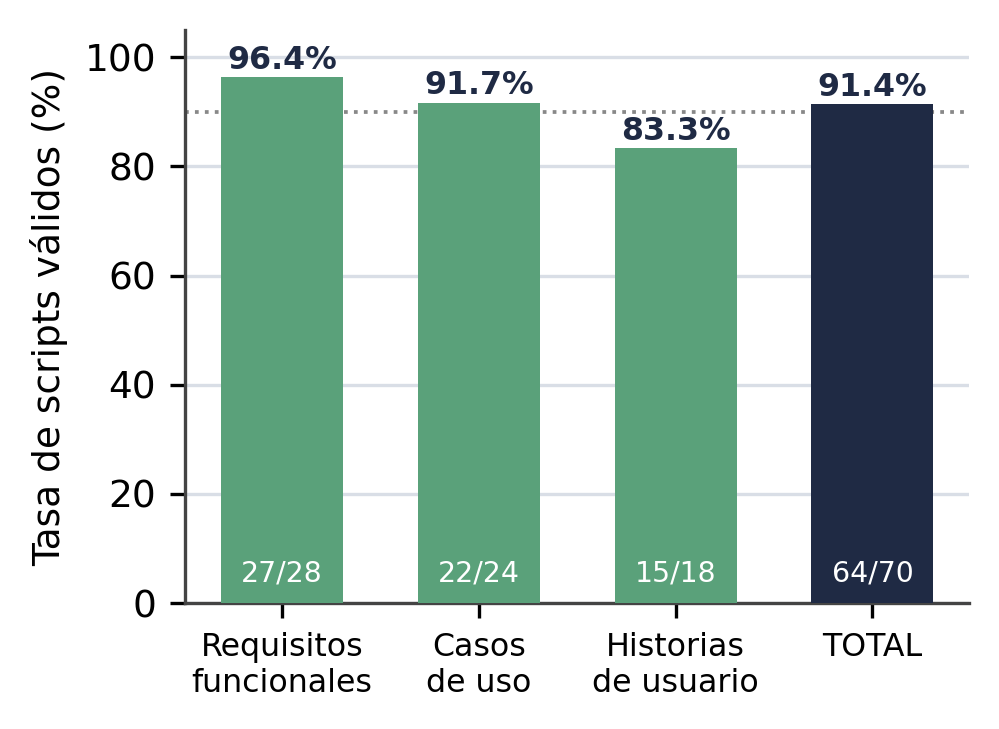
\includegraphics[width=0.92\columnwidth]{fig_generation.png}
		\caption{Tasa de scripts válidos por tipo de especificación (n\,=\,70 intentos). La etiqueta interior indica válidos/intentos.}
		\label{fig:generacion}
	\end{figure}
	
	\subsection{Usabilidad y aceptación tecnológica}
	\label{subsec:sustam}
	
	Los 25 participantes completaron las cuatro tareas en un tiempo medio de 42,0 minutos (DE\,=\,8,2). El puntaje SUS promedio fue de 74,82/100 (DE\,=\,6,18; mínimo 62,5; máximo 85,0), que supera el umbral de ``Bueno'' (68 puntos) de la escala de Bangor et~al. y sitúa a la herramienta por encima del promedio de los sistemas evaluados con este instrumento; el 76\,\% de los participantes otorgaron calificaciones de ``Bueno'' o ``Excelente'' \cite{bangor2009sus}. En cuanto a la aceptación tecnológica, los cuatro constructos TAM superaron el umbral de 3,5/5, como se observa en la Tabla~\ref{tab:tam} y en la Fig.~\ref{fig:tam}: Utilidad Percibida (4,14) e Intención de Uso (4,08) obtuvieron los valores más altos, mientras que Confianza en Resultados (3,76) fue el constructo más próximo al umbral, reflejando la incertidumbre de los participantes respecto de la fiabilidad del código generado por IA. El instrumento presentó una consistencia interna adecuada, con un coeficiente Alfa de Cronbach global de 0,883 y valores por constructo superiores a 0,79. El análisis de correlaciones de Pearson mostró que la asociación más fuerte se produce entre Utilidad Percibida e Intención de Uso (r\,=\,0,711; p\,<\,0,01), lo que confirma el supuesto central del modelo TAM.
	
	\begin{table}[!t]
		\caption{Estadística descriptiva y fiabilidad por constructo TAM (n\,=\,25)}
		\label{tab:tam}
		\centering
		\small
		\setlength{\tabcolsep}{3pt}
		\begin{tabular}{@{}lccccc@{}}
			\toprule
			\textbf{Constructo} & \textbf{Ítems} & \textbf{Media} & \textbf{DE} & \textbf{$\alpha$} & \textbf{Interp.} \\
			\midrule
			Utilidad Percibida (PU)   & 5 & 4,14 & 0,56 & 0,847 & Alta \\
			Facilidad de Uso (PEOU)   & 4 & 4,02 & 0,63 & 0,812 & Alta \\
			Confianza Result. (CR)    & 4 & 3,76 & 0,71 & 0,798 & Mod.-Alta \\
			Intención de Uso (IU)     & 3 & 4,08 & 0,60 & 0,831 & Alta \\
			\midrule
			\textbf{Global}           & \textbf{16} & \textbf{4,00} & \textbf{0,63} & \textbf{0,883} & \textbf{Alta} \\
			\bottomrule
		\end{tabular}
	\end{table}
	
	\begin{figure}[!t]
		\centering
		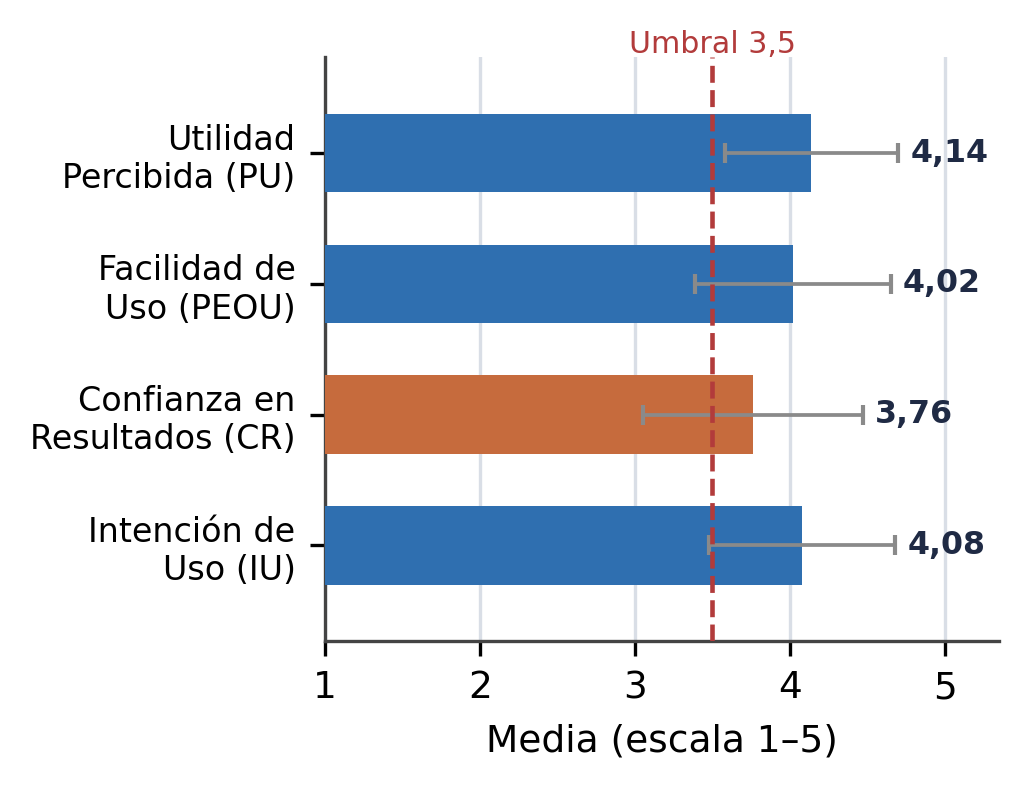
\includegraphics[width=0.92\columnwidth]{fig_tam.png}
		\caption{Media por constructo TAM frente al umbral de aceptación de 3,5. Las barras muestran la desviación estándar.}
		\label{fig:tam}
	\end{figure}
	
	\subsection{Calidad de las pruebas generadas}
	\label{subsec:calidad}
	
	La evaluación experta arrojó una calidad media global de 4,08/5,0 sobre los cinco criterios de la rúbrica, como muestran la Tabla~\ref{tab:calidad} y la Fig.~\ref{fig:calidad}. Los criterios mejor valorados fueron claridad (4,3) y completitud (4,2), calificados como ``Muy bueno'', mientras que la viabilidad de ejecución (3,9) resultó el criterio más próximo al umbral, lo que sugiere oportunidades de mejora en la precisión de las aserciones respecto de las condiciones de la especificación de origen. Desagregando por tipo de prueba, las pruebas unitarias generadas desde requisitos funcionales alcanzaron la calidad más alta (4,24), seguidas de las pruebas de integración desde casos de uso (4,08) y las pruebas de sistema desde historias de usuario (3,92), diferencia atribuible a la mayor ambigüedad inherente a las historias de usuario complejas.
	
	\begin{table}[!t]
		\caption{Calidad de las pruebas por criterio (escala 1--5, n\,=\,10 expertos)}
		\label{tab:calidad}
		\centering
		\small
		\begin{tabular}{@{}lccc@{}}
			\toprule
			\textbf{Criterio} & \textbf{Media} & \textbf{DE} & \textbf{Interpretación} \\
			\midrule
			Completitud            & 4,2 & 0,45 & Muy bueno \\
			Claridad               & 4,3 & 0,42 & Muy bueno \\
			Trazabilidad           & 4,0 & 0,58 & Bueno \\
			Viabilidad de ejecución & 3,9 & 0,67 & Bueno \\
			Cobertura de escenarios & 4,0 & 0,61 & Bueno \\
			\midrule
			\textbf{Media global}  & \textbf{4,08} & \textbf{0,55} & \textbf{Muy bueno} \\
			\bottomrule
		\end{tabular}
	\end{table}
	
	\begin{figure}[!t]
		\centering
		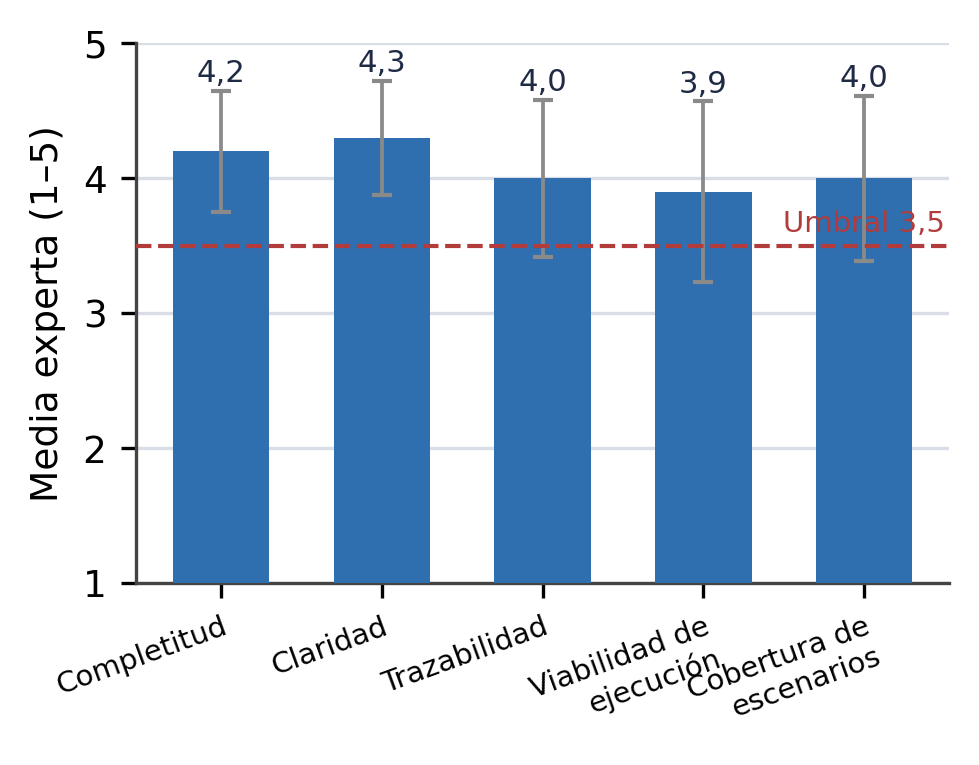
\includegraphics[width=0.92\columnwidth]{fig_quality.png}
		\caption{Calidad media por criterio evaluada por expertos frente al umbral de 3,5.}
		\label{fig:calidad}
	\end{figure}
	
	%% ------------------------------------------------------------------------
	\section{Discusión}
	\label{sec:discusion}
	
	Los hallazgos de este trabajo se interpretan a la luz del cuerpo de 108 estudios primarios incluidos en la revisión sistemática \cite{p001,p002,p003,p004,p005,p006,p007,p008,p009,p010,p011,p012,p013,p014,p015,p016,p017,p018,p019,p020,p021,p022,p023,p024,p025,p026,p027,p028,p029,p030,p031,p032,p033,p034,p035,p036,p037,p038,p039,p040,p041,p042,p043,p044,p045,p046,p047,p048,p049,p050,p051,p052,p053,p054,p055,p056,p057,p058,p059,p060,p061,p062,p063,p064,p065,p066,p067,p068,p069,p070,p071,p072,p073,p074,p075,p076,p077,p078,p079,p080,p081,p082,p083,p084,p085,p086,p087,p088,p089,p090,p091,p092,p093,p094,p095,p096,p097,p098,p099,p100,p101,p102,p103,p104,p105,p106,p107,p108}, que delimita el estado del arte en la captura estructurada de requisitos y su relación con la generación automática de pruebas. Los resultados aportan evidencia de que la generación estructurada del estado inicial de las pruebas asistida por un LLM es viable y bien aceptada. La tasa global de scripts válidos del 91,4\,\% es superior al 78\,\% reportado por \emph{Pytester} para la generación de casos de prueba ejecutables desde texto en lenguaje natural \cite{takerngsaksiri2025pytester}, lo que sugiere que la combinación de captura estructurada de especificaciones y validación sintáctica automática mediante AST constituye una mejora metodológica concreta respecto de enfoques que operan sobre texto libre sin verificación integrada. Este hallazgo es coherente con la evidencia de la literatura de que la calidad de la especificación de entrada es el factor determinante de la coherencia de las pruebas generadas: el mejor desempeño se obtuvo precisamente en los requisitos funcionales, más estructurados, y el menor en las historias de usuario, más ambiguas \cite{wang2024survey,yang2024evaluation}.
	
	El posicionamiento de TDDMachine en la etapa \emph{Red} del ciclo la diferencia de herramientas como \emph{ChatUniTest}, \emph{TestSpark} o \emph{Pynguin}, orientadas a generar pruebas desde código fuente existente \cite{chen2024chatunitest,sapozhnikov2024testspark,lukasczyk2022pynguin}. Al intervenir antes de que exista código de producción, la herramienta se alinea con el principio fundamental del TDD de escribir primero la prueba y, con ello, con la evidencia de que anticipar las pruebas reduce la densidad de defectos y el esfuerzo de corrección posterior a la entrega \cite{nagappan2008tdd,rafique2013meta,erdogmus2005testfirst}. Los niveles de usabilidad (SUS\,=\,74,82) y de aceptación (todos los constructos TAM por encima del umbral, con la Utilidad Percibida como predictor más fuerte de la Intención de Uso) indican, además, que la herramienta es percibida como útil y fácil de usar por usuarios sin experiencia previa en \texttt{pytest}, lo que aborda directamente la barrera de adopción del TDD asociada a la curva de aprendizaje del \emph{testing} \cite{ghafari2020inconclusive,bangor2009sus,davis1989tam}. El puntaje SUS obtenido es comparable al de otras herramientas de soporte al desarrollo evaluadas con el mismo instrumento en la línea de investigación del grupo \cite{guerrero2025tddtool}.
	
	Entre las amenazas a la validez deben considerarse las siguientes. La validez externa está limitada por una muestra compuesta exclusivamente por estudiantes de un mismo semestre y por un conjunto de especificaciones que no cubre todos los dominios de aplicación posibles; la generalización a profesionales y a contextos industriales requiere estudios adicionales. La validez de constructo del criterio de viabilidad de ejecución está acotada por su evaluación mediante inspección estructural del código y no mediante su ejecución efectiva, decisión coherente con el alcance de la herramienta ---que cubre la etapa \emph{Red} y no la \emph{Green}--- pero que impide afirmar la ejecutabilidad en \emph{pipelines} reales de integración continua. Finalmente, las mediciones corresponden a una primera sesión de interacción, por lo que la estabilidad de las percepciones en un uso sostenido queda por confirmar.
	
	%% ------------------------------------------------------------------------
	\section{Conclusiones}
	\label{sec:conclusiones}
	
	Este trabajo presentó TDDMachine, una herramienta CASE que automatiza la generación del estado inicial de las pruebas ---la etapa \emph{Red} del ciclo TDD--- a partir de especificaciones estructuradas y mediante el modelo de lenguaje Claude 3.5 Sonnet, con validación sintáctica automática del código generado por análisis del AST de Python. La herramienta, cuyos requisitos se derivaron de una revisión sistemática de 108 estudios primarios y cuya pila tecnológica se seleccionó por evaluación multicriterio, produjo scripts \texttt{pytest} válidos en el 91,4\,\% de los intentos, alcanzó una calidad media evaluada por expertos de 4,08/5,0, obtuvo un puntaje SUS de 74,82/100 y superó el umbral de aceptación tecnológica en los cuatro constructos TAM. En conjunto, estos resultados validan la hipótesis central del proyecto: es posible construir una herramienta CASE que, a partir de especificaciones estructuradas y empleando un LLM como motor de generación y el AST como mecanismo de control de calidad, automatice la generación del estado inicial de pruebas para la metodología TDD.
	
	En el plano teórico, el estudio conecta dos marcos previamente tratados por separado: el principio \emph{test-first} del TDD ---escribir la prueba antes que el código--- y la teoría de aceptación tecnológica que explica la adopción de una herramienta a partir de su utilidad y facilidad de uso percibidas. Al situar la generación asistida por LLM en la etapa \emph{Red} y evidenciar que esa anticipación es percibida como útil y usable, el trabajo aporta un puente empírico entre la anticipación de pruebas como práctica de calidad y la aceptación de las herramientas que la soportan. La principal contribución es, por tanto, empírica y metodológica: la evidencia de que anteponer una captura estructurada de requisitos a la generación por LLM, y verificar el resultado mediante AST, mejora la proporción de scripts válidos respecto de enfoques que operan sobre texto libre, y de que este proceso es percibido como útil y usable por desarrolladores noveles. Como líneas de trabajo futuro se plantean: la extensión de la validación mediante la ejecución real de los scripts en entornos controlados para medir la tasa de éxito en la etapa \emph{Green}; la incorporación de instrucciones explícitas en los \emph{prompts} para forzar escenarios negativos y de valor límite, atendiendo a la principal recomendación de los expertos; la ampliación de la evaluación a profesionales y a mayor diversidad de dominios; y la preparación de la versión en inglés del manuscrito para su envío a \emph{Enfoque UTE}.
	
	%% ------------------------------------------------------------------------
	%% DECLARACIONES OBLIGATORIAS DE ENFOQUE UTE (2026)
	%% ------------------------------------------------------------------------
	\seccionetica{%
		Both evaluation studies involved voluntary participants and followed an ethics protocol. Every participant provided written informed consent before any activity; the consent form stated the voluntary nature of participation, its exclusively academic purpose, the tasks to be performed, the data to be collected, the confidentiality guarantees, the right to withdraw at any time without penalty, and the data-retention period. The collected data were handled confidentially, stored in access-restricted digital forms, and reported only in aggregate, without individual identification.
	}
	
	\seccionfunding{%
		This research received no external funding.
	}
	
	\seccionconflicto{%
		The authors declare that they have no conflict of interest.
	}
	
	\seccioniadeclaracion{%
		The authors declare that generative artificial intelligence tools were used to assist in language editing and in the drafting and structuring of this manuscript. The core scientific content, the design of the tool, the experimental design, the data collection and the analysis of results are the sole work and responsibility of the authors, who take full responsibility for the content of the manuscript.
	}
	
	%% ------------------------------------------------------------------------
	\bibliographystyle{IEEEtran}
	\bibliography{references}
	
\end{document}